\documentclass[english,12pt,presentation]{beamer}
\usepackage{graphicx}
%\usepackage{movie15}
\usepackage{beamerthemesplit}
%\setbeameroption{show notes on second screen=right}
\usetheme{Bergen}
%\useinnertheme{circles}
\useinnertheme{inmargin}
\useoutertheme{infolines}
\usecolortheme{spruce}
\title{Emacs as a potential tool for Drupal Development and Management}
\subtitle{HTML, CSS, PHP, LISP, JS, Python, etc}
\author{Aaron Bello, aaron@hosttor.com, @hosttor}
\date{\ August 22 2015}

\begin{document}
\begin{frame}{Drupal Camp, Yale University}
\begin{figure}
\centering

\includegraphics[width=80]{images/logo.png}
\end{figure}
\titlepage
\end{frame}

\begin{frame}{Proudly Sponsored By}
\begin{figure}
\centering

\includegraphics[width=220]{images/agaric.png}
\end{figure}
\end{frame}

\begin{frame}{What is GNU Emacs?}
\begin{itemize}
\pause \item A powerful tool for all programmers. It is extensible, customizable, self-documenting real-time display editor. 
\pause \item Writen in Lisp. Lisp was developed at MIT for research in artificial intelligence. 
\pause \item Use emacs to write in many different human languages and programming or markup languages.
\pause \item Supported OS are GNU/Linux, Mac OS X, MS Windows, Solaris
\pause \item Download GNU Emacs at gnu.org/software/emacs
\pause \item Ctrl-h followed by t. For Tutorial
\end{itemize}
\end{frame}

\begin{frame}{Emacs Supported Technologies}
\begin{itemize}
\pause \item HTML, CSS and Javascript
\pause \item Python, Django
\pause \item Java
\pause \item Lisp
\pause \item C or C$++$
\pause \item Arduino
\pause \item Vi/Vim
\pause \item Swift
\pause \item And many more...
\end{itemize}
\end{frame}

\begin{frame}{Thanks to Free Software Foundation}
\begin{figure}
\centering

\includegraphics[width=220]{images/fsf.png}
\end{figure}
\end{frame}

\begin{frame}{Why Emacs For Drupal Development?}
\begin{itemize}
\pause \item Save time and increase productivity
\pause \item The best industry tools for professionals
\pause \item It is Free Software. No licence fees
\pause \item You can modify the source code oppose to what you paid for with limitations.
\pause \item You can share the software among your family, friends and anyone interested in Free Software.
\pause \item Huge community with users worldwide.
\end{itemize}
\end{frame}

\begin{frame}{Powerful Brands Using Drupal}
\begin{figure}
\centering
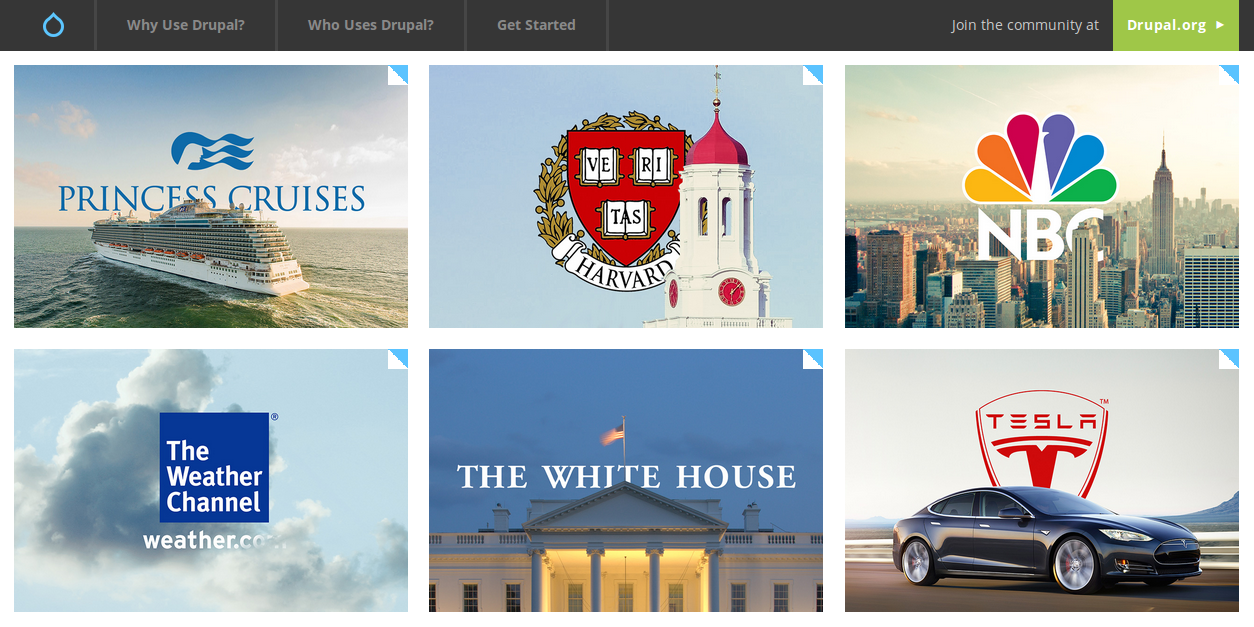
\includegraphics[width=220]{images/drupaluser.png}
\end{figure}
\end{frame}

\begin{frame}{Powerful Brands using Drupal}
\begin{itemize}
\pause \item Stanford Law School
\pause \item Brown University
\pause \item Yale University
\pause \item University of Oxford
\pause \item Bentley University
\pause \item PUMA - PUMA.COM
\pause \item CJ Affliate By Conversant - CJ.COM
\pause \item The University of Tennessee and other universities
\pause \item Governments, Corporations and Organizations around the world have also adopted Drupal
\end{itemize}
\end{frame}

\begin{frame}{Demostration Time}
\begin{itemize}
\pause \item There are so many packages available to download.
\pause \item Use Alt-x list-packages to see all packages.
\end{itemize}
\begin{figure}
\centering

\includegraphics[width=220]{images/altx.png}
\end{figure}
\end{frame}

\begin{frame}{Demostration Time}
\begin{itemize}
\pause \item org-mode, org-agenda
\pause \item weather, phases-of-moon, dictionary, holiday, chess, doctor, macroc
\pause \item auto-complete, emmet, yasnipet, rainbow, show css
\pause \item weblogger-setup-weblog. Require blogger API. visit abc.com/xmlrpc.php
\pause \item You can create your own package using Emacs Lisp code or GUI.
\end{itemize}
\end{frame}

\begin{frame}{How I Use Emacs}
\begin{itemize}
\pause \item Twitter, IRC, LaTex, Secure Password, HTML, CSS, PHP, JS
\pause \item SSH, RSYNC, FTP, SCP, etags for Drupal Website
\pause \item Drupal mode is an advanced minor mode for development and management
\pause \item Write code that adheres to drupal coding standards.
\pause \item Search documentation for the symbol at point
\pause \item python, Java, vi/vim, C or C$++$, Lisp, Arduino and many more...
\end{itemize}
\end{frame}

\begin{frame}{Thank you all for coming}
\item Thank you! Thank you!! Thank you!!!
\end{frame}

\begin{frame}{QUESTIONS?}
\begin{figure}
\centering

\includegraphics[width=220]{images/q.png}
\end{figure}
\end{frame}
\end{document}

